\documentclass{jsarticle}
\date{\today}
\title{初めてのtex}
\usepackage[dvipdfmx]{graphicx}

\begin{document}
\maketitle
\section {自己紹介}
\subsection {--- 氏名:林 実樹}

\subsection {--- 生年月日:1999:11:11}
\section {画像の利用}
% 図の挿入
\begin{figure}[htbp]
\begin{center}
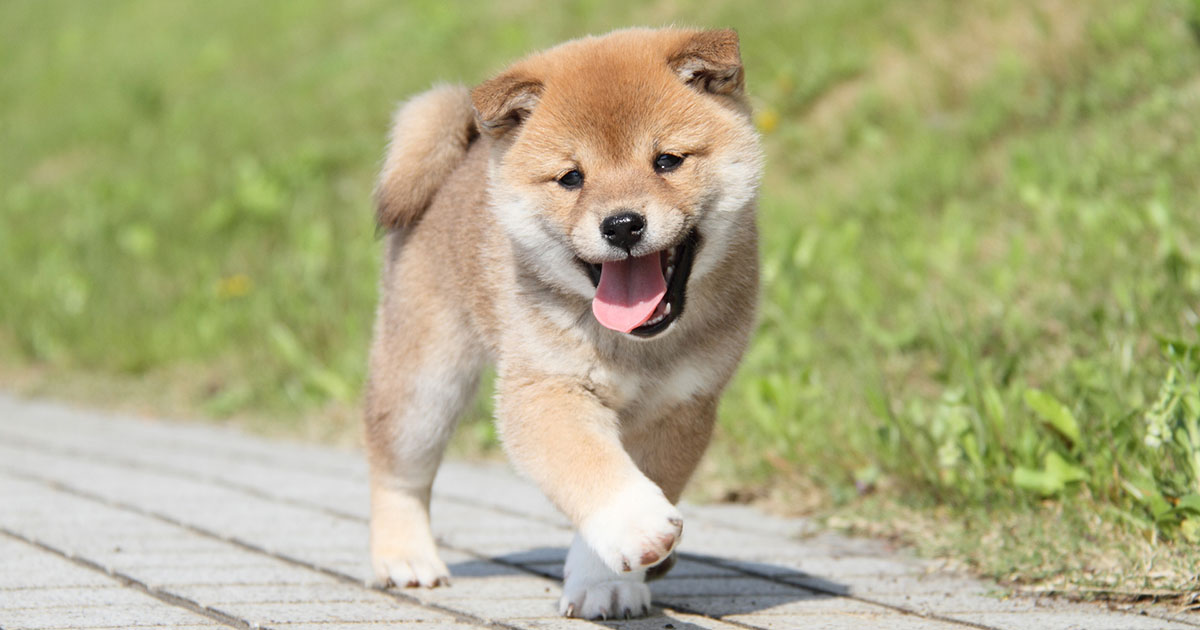
\includegraphics[width=100mm]{img_dog.png}
\caption{犬}
\end{center}
\end{figure}

\section {表を作成する}
%表の挿入
\begin{table}[htbp]
  \centering
  \begin{tabular}{l|c|r}
    1 & 2 & 3 \\ \hline\hline
    sin & cos & tan \\
    apple & pine & banana \\ \hline
  \end{tabular}
  \caption{fugafuga}
  \label{tb:fugafuga}
\end{table}

\begin{thebibliography}{99}
  \item 奥村晴彦,黒木裕介『\LaTeXe 美文書作成入門』第7版(技術評論社,2017)
  \item ……
\end{thebibliography}

\end{document}